\chapter{Projekt aplikacji}

\section{Interfejs użytkownika}
\subsection{Menu}

\begin{figure}
    \centering
    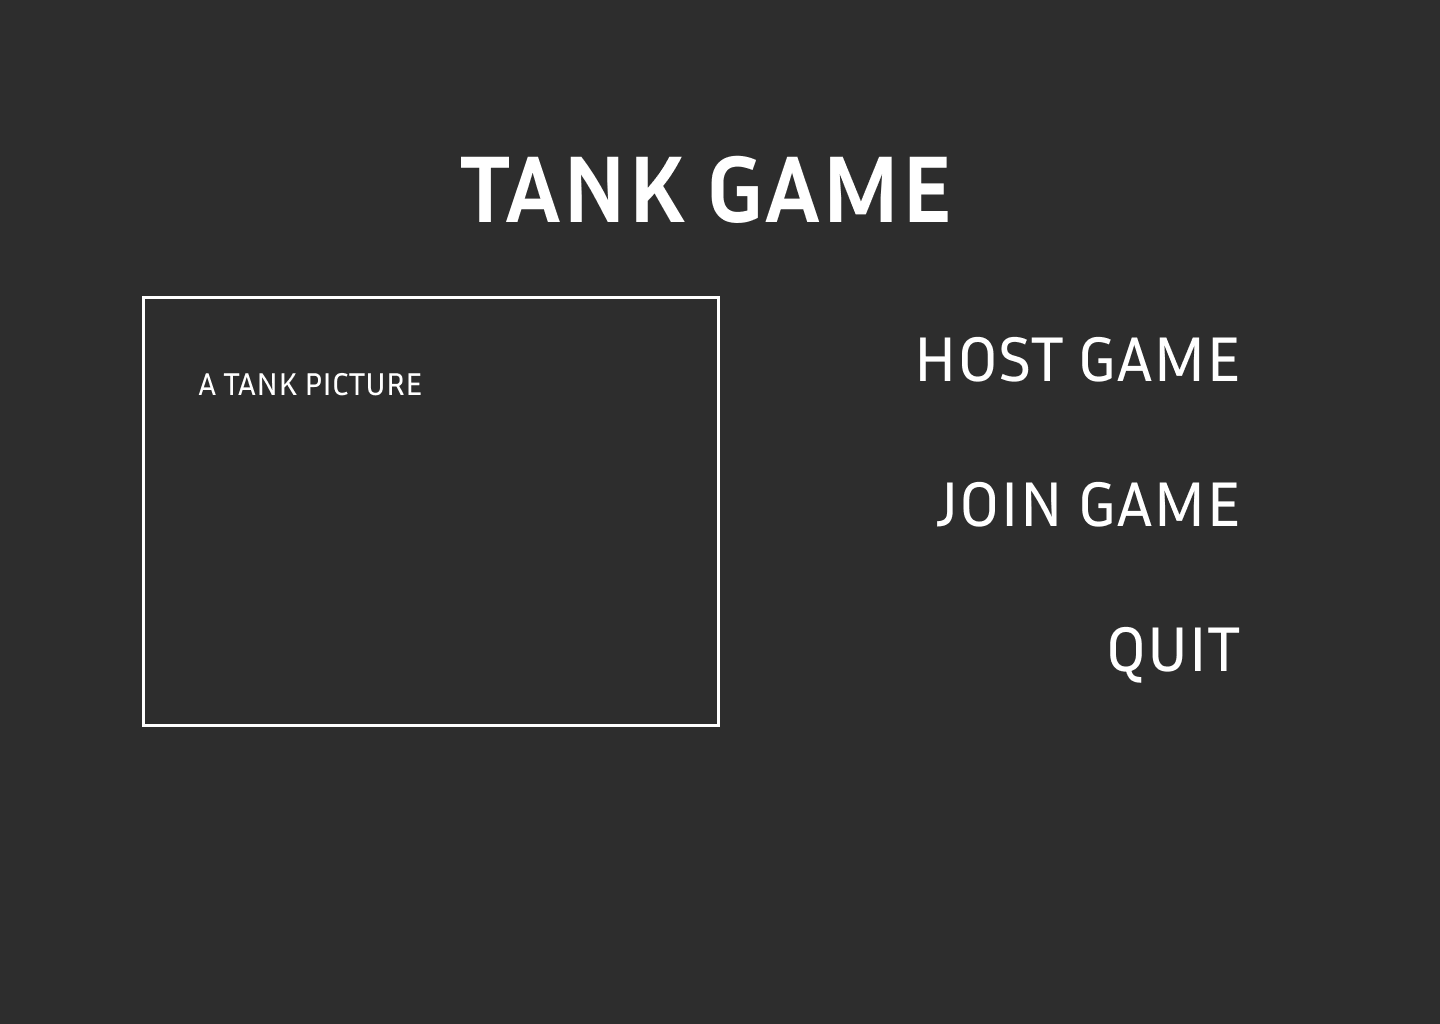
\includegraphics[width=.8\linewidth]{Images/design/Main Menu.png}
    \caption{Projekt menu głównego.}
    \label{fig:main_menu}
\end{figure}

\begin{figure}
    \centering
    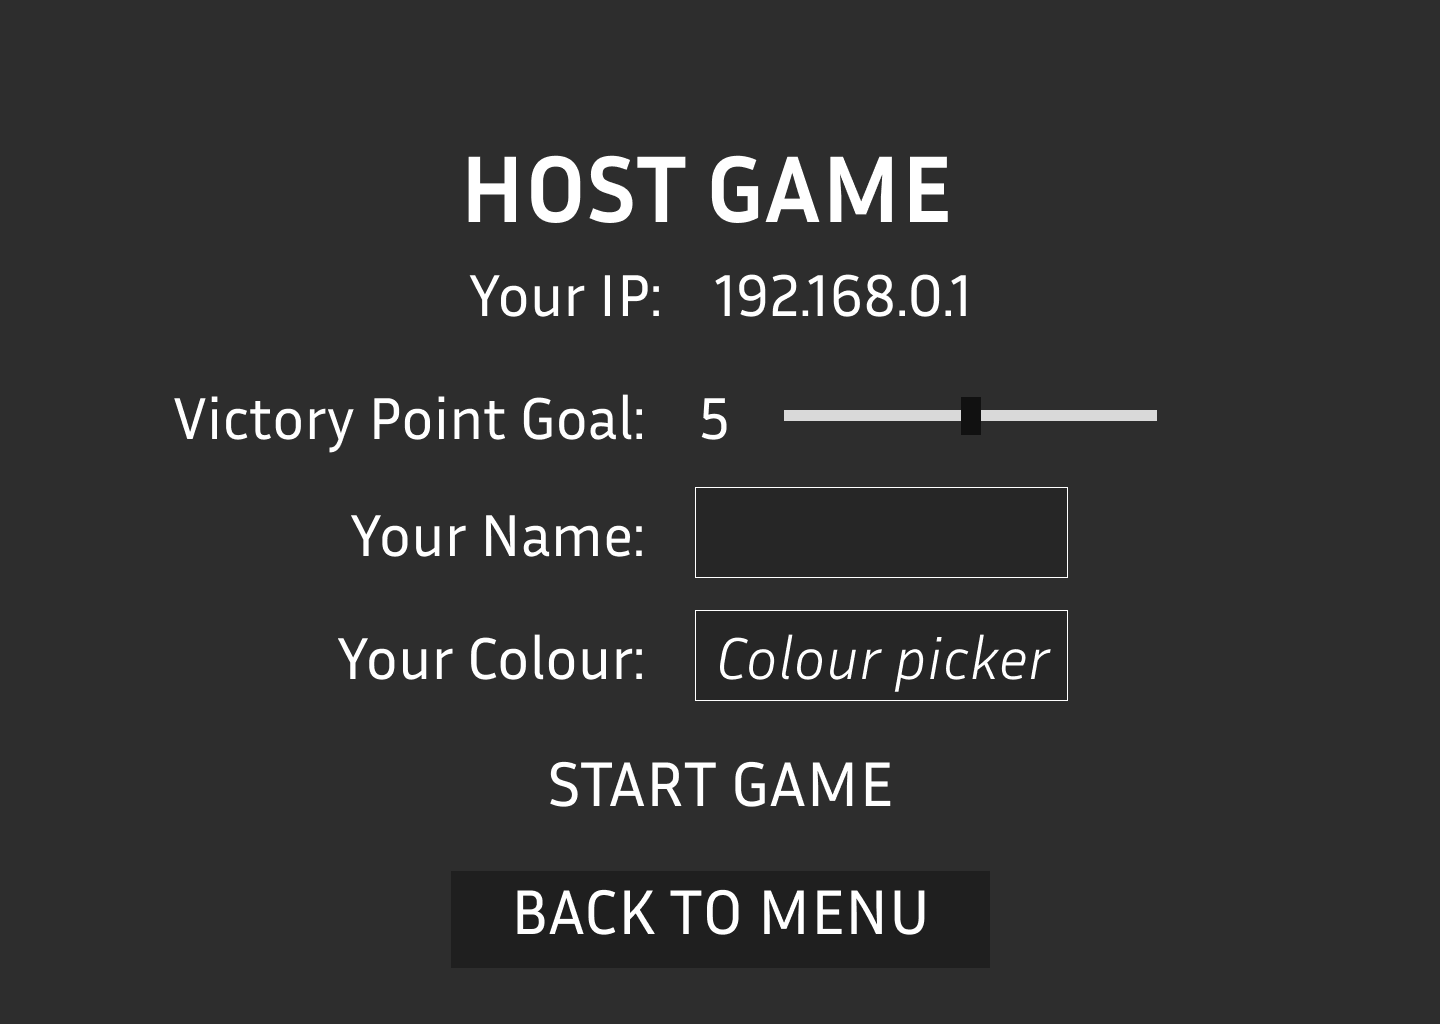
\includegraphics[width=.8\linewidth]{Images/design/Host Menu.png}
    \caption{Projekt menu hosta.}
    \label{fig:host_menu}
\end{figure}

\begin{figure}
    \centering
    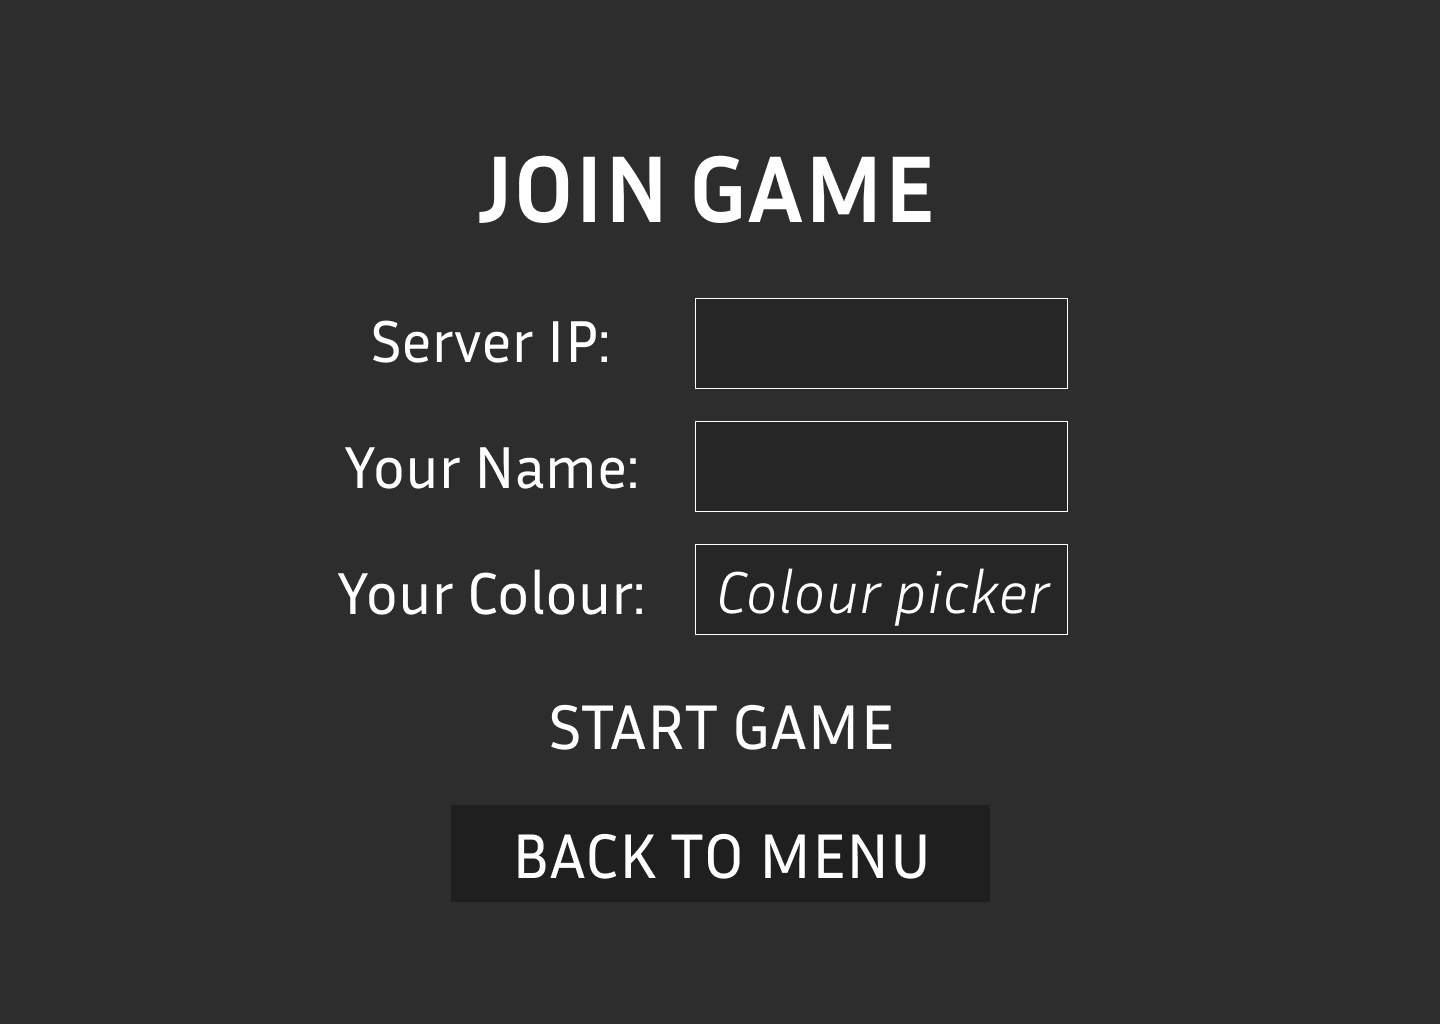
\includegraphics[width=.8\linewidth]{Images/design/Join Menu.png}
    \caption{Projekt menu dołączającego gracza.}
    \label{fig:join_menu}
\end{figure}

\begin{figure}
    \centering
    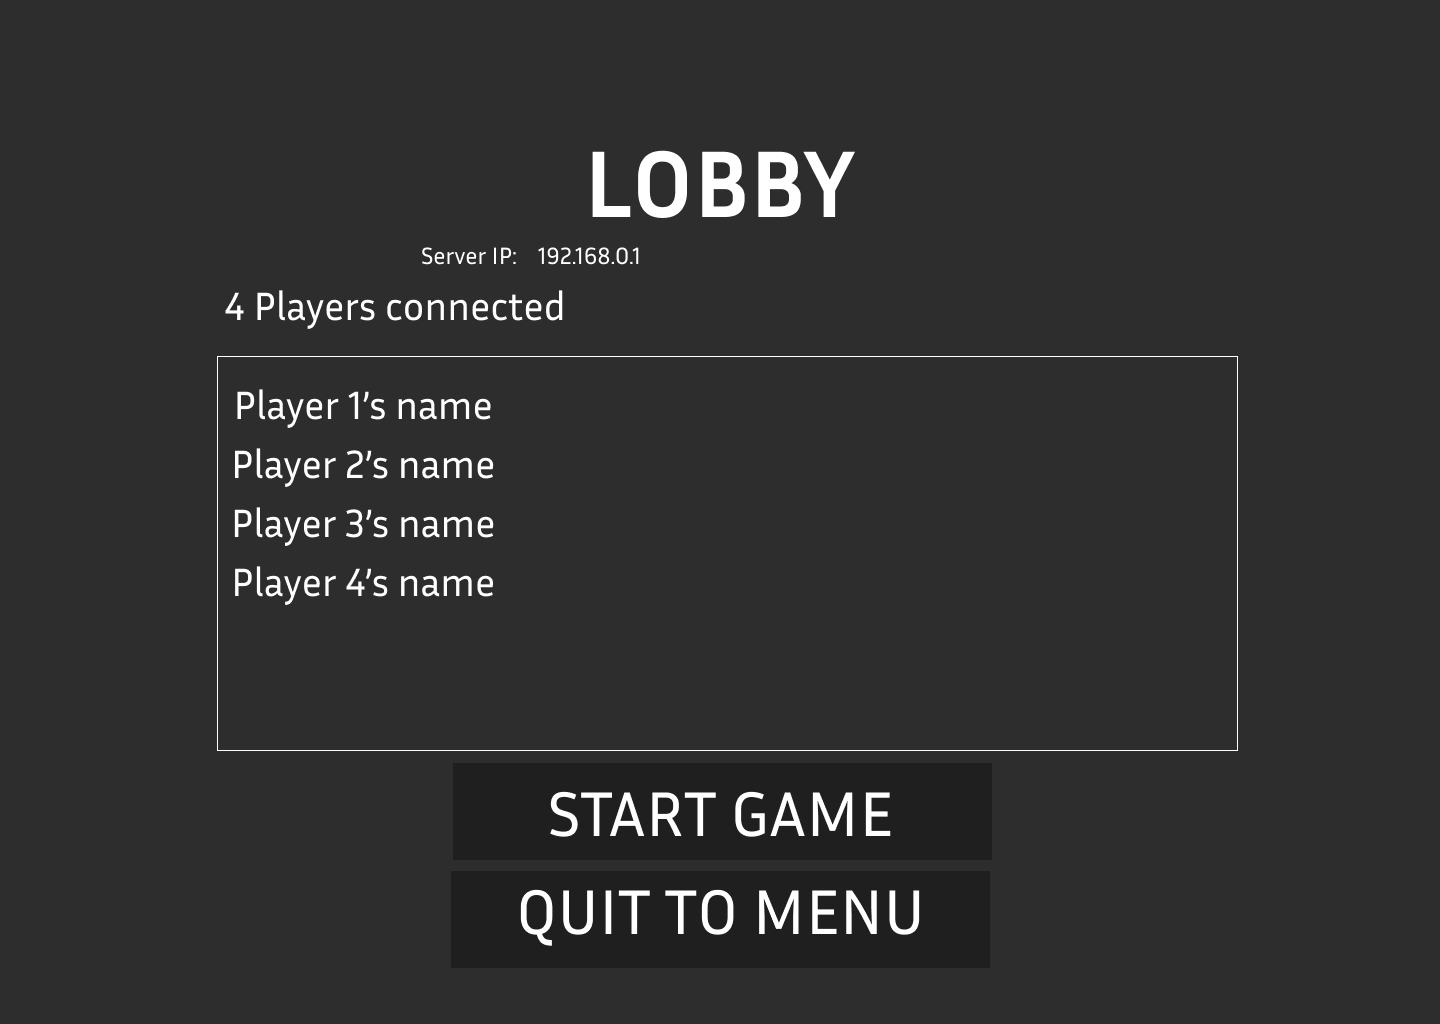
\includegraphics[width=.8\linewidth]{Images/design/Lobby Menu.png}
    \caption{Projekt menu poczekalni.}
    \label{fig:lobby_menu}
\end{figure}

\begin{figure}
    \centering
    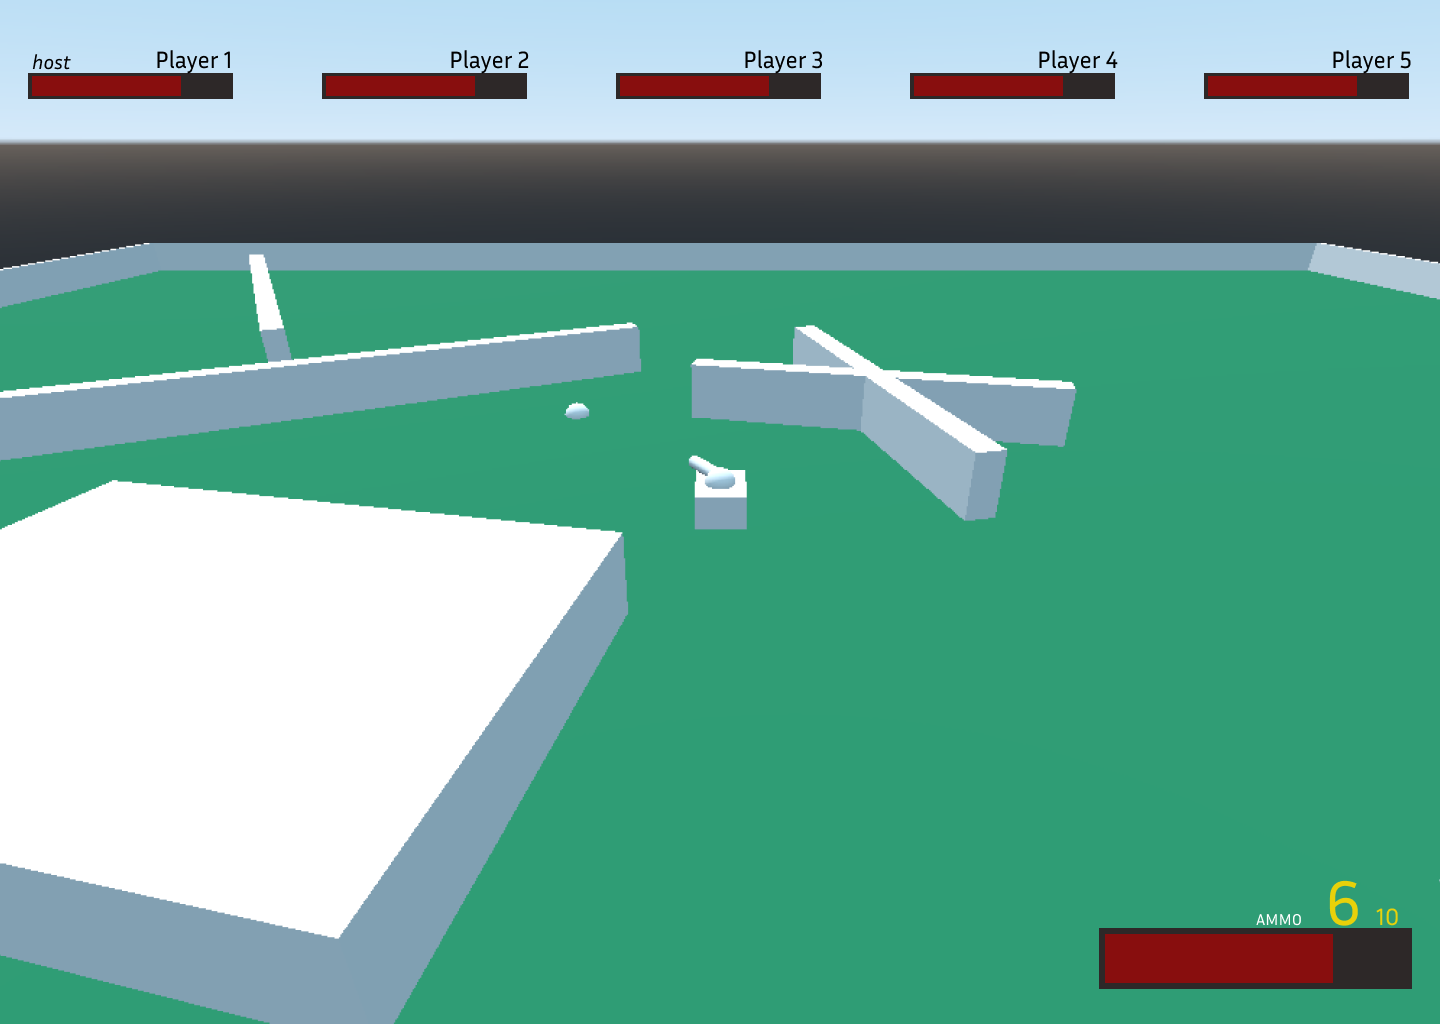
\includegraphics[width=.8\linewidth]{Images/design/Game View.png}
    \caption{Projekt interfejsu HUD.}
    \label{fig:game_view}
\end{figure}

\begin{figure}
    \centering
    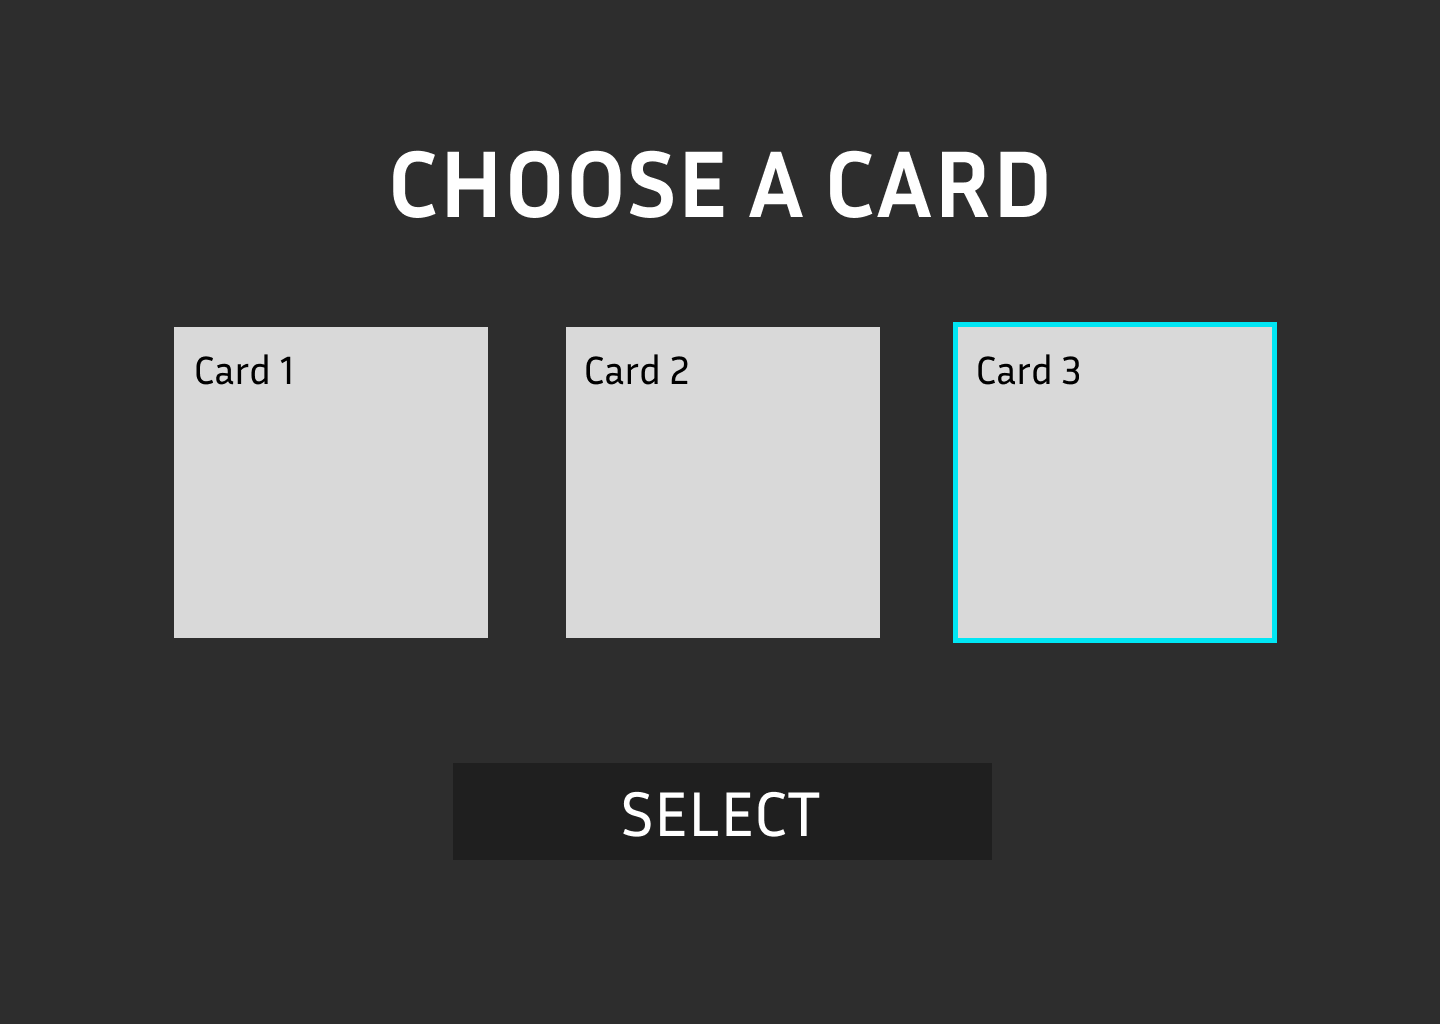
\includegraphics[width=.8\linewidth]{Images/design/Cards Menu.png}
    \caption{Projekt menu wyboru kart.}
    \label{fig:cards_menu}
\end{figure}

\begin{figure}
    \centering
    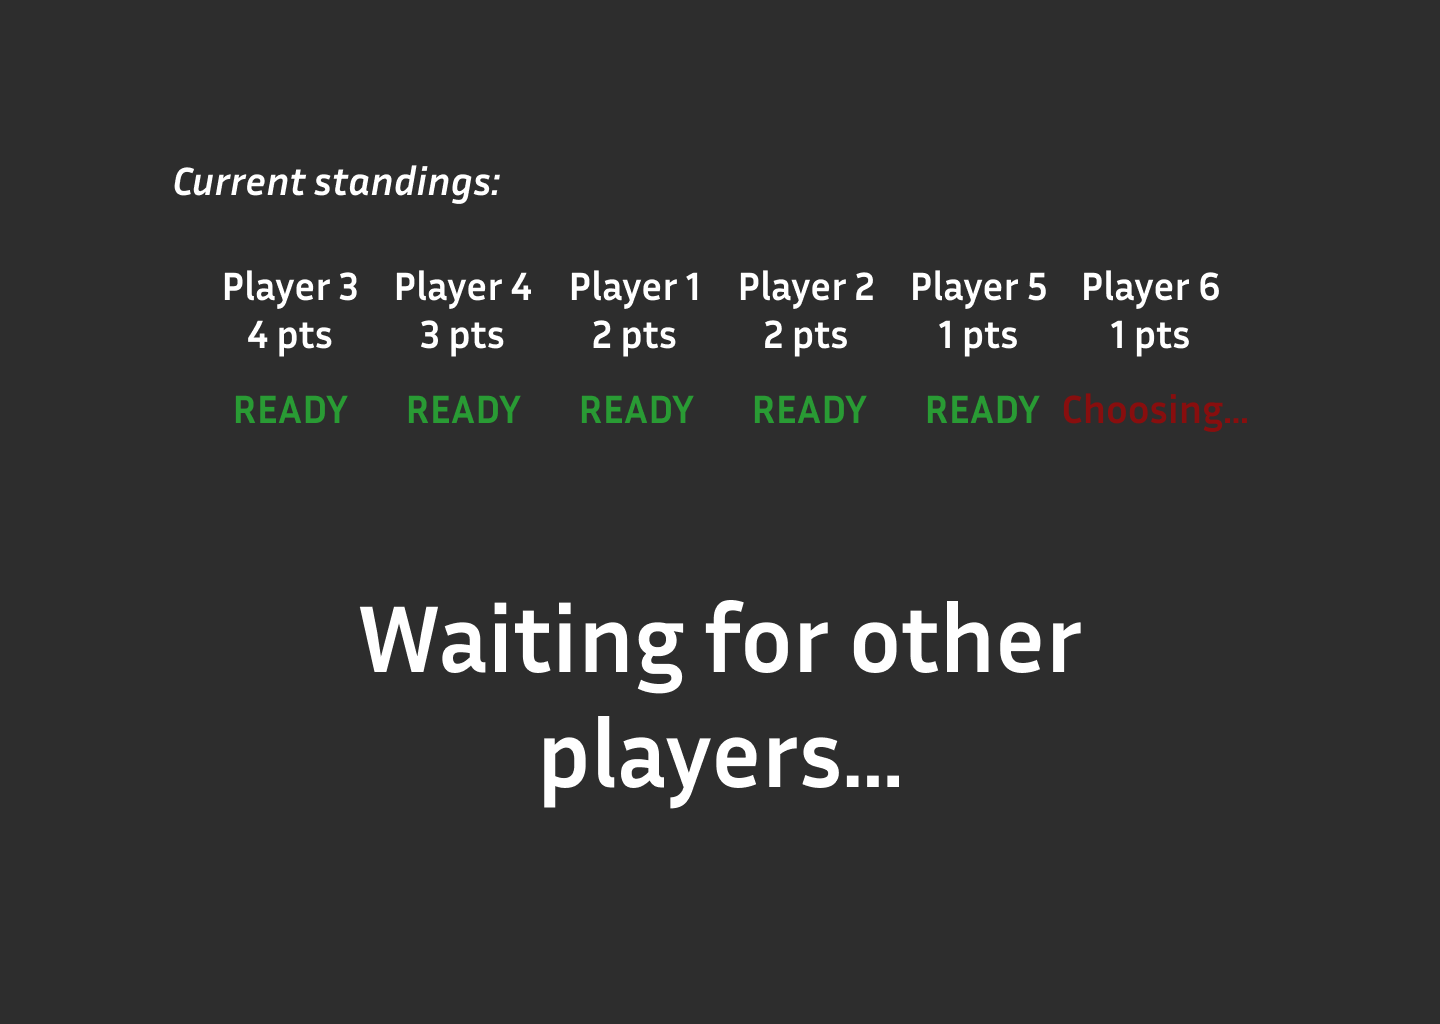
\includegraphics[width=.8\linewidth]{Images/design/Waiting Menu.png}
    \caption{Projekt menu oczekiwania między turami.}
    \label{fig:waiting_menu}
\end{figure}

\begin{figure}
    \centering
    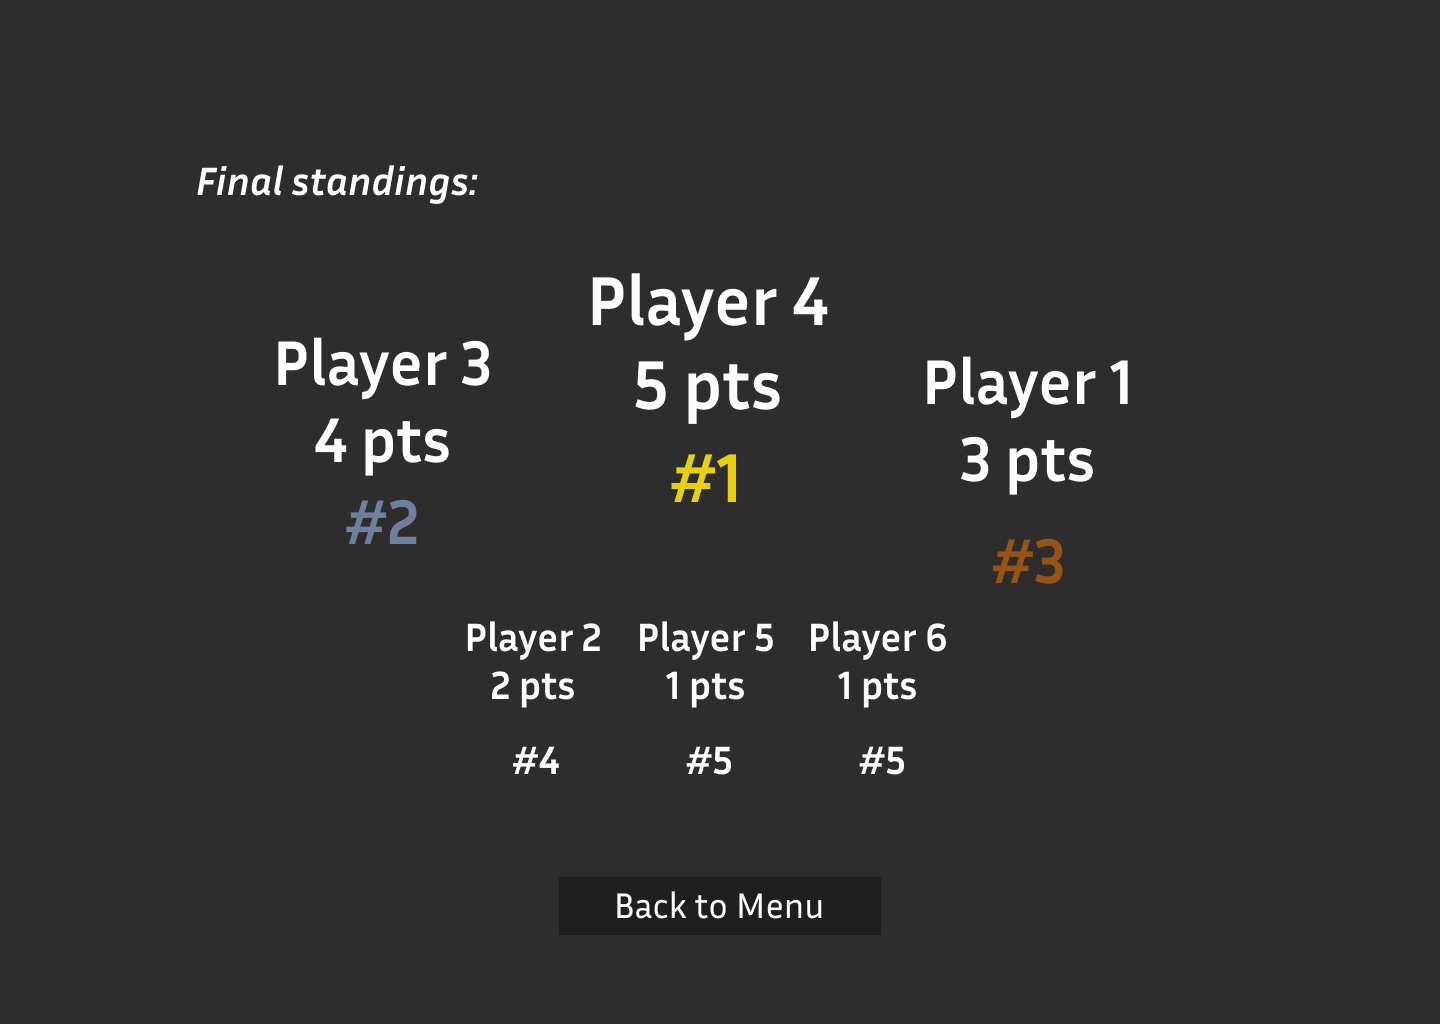
\includegraphics[width=.8\linewidth]{Images/design/Final Menu.png}
    \caption{Projekt ekranu po zakończeniu rozgrywki.}
    \label{fig:final_menu}
\end{figure}

\subsection{HUD}

\subsection{Schemat sterowania}

\begin{table}
    \small
    \centering
    \caption{Schemat sterowania}
    \label{tab:steering}
    \begin{tabularx}{\linewidth}{|c|c|X|}
        \hline
        Nazwa akcji & Przypisany przycisk & Opis czynności\\
        \hline \hline
        Forward & W & Poruszanie do przodu. \\
        \hline
        Back & S & Poruszanie do tyłu. \\
        \hline
        Left & A & Obrót postaci w lewo, przeciwnie do ruchu wskazówek zegara.\\
        \hline
        Right & D & Obrót postaci w prawo, zgodnie z ruchem wskazówek zegara.\\
        \hline 
        MainAction & Lewy przycisk myszy & Akcja podstawowa - strzał.\\
        \hline
    \end{tabularx}
\end{table}

\section{Implementacja mechanik}
\subsection{Model danych postaci}
\subsection{Poruszanie}
\subsection{Strzelanie}
\subsubsection{Wydarzenia po trafieniu}
\subsection{Zdrowie}
\subsection{Rundy}
\subsection{Karty ulepszeń}


\section{System sieciowy}
\subsection{Poczekalnia}
\subsection{Proces hostowania gry}
\subsection{Proces dołączania do gry}
\subsection{Przepływ danych w grze}